\documentclass{article}

%Package Part
\usepackage{relsize,setspace}  % used by latex(describe( ))
\usepackage{url}               % used in bibliography
\usepackage[superscript,nomove]{cite} % use if \cite is used and superscripts wanted
% Remove nomove if you want superscripts after punctuation in citations
\usepackage{lscape}            % for landscape mode tables
\textwidth 6.75in              % set dimensions before fancyhdr 
\textheight 9.25in
\topmargin -.875in
\oddsidemargin -.125in
\evensidemargin -.125in
\usepackage{fancyhdr}          % this and next line are for fancy headers/footers
\pagestyle{fancy}
\newcommand{\bc}{\begin{center}}  % abbreviate
\newcommand{\ec}{\end{center}}

\usepackage{Sweave}
\begin{document}

\Sconcordance{concordance:test.tex:test.Rnw:%
1 18 1 1 0 14 1 1 21 4 1 1 2 31 0 1 1 24 0 1 1 14 0 1 1 27 0 1 2 2 1 1 %
6 1 2 5 1 1 2 1 3 1 2 4 1 1 2 1 3 1 2 2 1 1 2 1 3 1 2 4 1 1 2 1 3 1 2 3 %
1 1 2 1 3 1 2 2 1 1 2 1 3 1 2 4 1 1 2 1 3 1 2 3 1 1 2 1 3 1 2 2 1 1 2 1 %
3 1 2 2 1}


%\SweaveOpts{width=6, height=4}


\title{Performance Analysis}
\author{}
\date{}

\setkeys{Gin}{width=1\textwidth}
\maketitle
%\tableofcontents


\section{Overview}
This documents go through performance of \verb|Foreign_1W_Mkt_cap|. Simulation period is from 2006-01-06 09:00:00 to 2013-01-04 09:00:00. The portfolio is composed with Large Caps (which hedge by Equity Trading Team in 'H' securities). Data source is WiseFN.

\subsection{Tables}
% latex table generated in R 2.15.2 by xtable 1.7-0 package
% Tue Jan 08 20:52:26 2013
\begin{table}[ht]
\begin{center}
\caption{Calendar Returns}
\begin{tabular}{rrrrrrrrr}
  \hline
 & 2006 & 2007 & 2008 & 2009 & 2010 & 2011 & 2012 & 2013 \\ 
  \hline
1 &  & -2.10 & -13.00 & 7.70 & -4.10 & 2.50 & 11.80 & -1.20 \\ 
  2 & 7.80 & 6.80 & 2.90 & -9.20 & 1.30 & -9.00 & -0.50 &  \\ 
  3 & 1.70 & 0.00 & 0.10 & 12.50 & 9.90 & 8.50 & -3.20 &  \\ 
  4 & 5.10 & 6.20 & 9.00 & 10.60 & -0.40 & 11.10 & -3.90 &  \\ 
  5 & -3.60 & 12.70 & -2.40 & 6.20 & -5.60 & -8.10 & -9.20 &  \\ 
  6 & 7.80 & 3.60 & -9.30 & 0.10 & 6.80 & 5.40 & 1.70 &  \\ 
  7 & -1.20 & 10.10 & -4.70 & 9.10 & -0.00 & -0.70 & 0.10 &  \\ 
  8 & 4.50 & -0.70 & -9.20 & 4.50 & -3.20 & -21.90 & 7.00 &  \\ 
  9 & 5.90 & 9.10 & -0.50 & 1.70 & 4.50 & -1.40 & 3.60 &  \\ 
  10 & -1.70 & 16.20 & -26.30 & -4.00 & 0.80 & 5.50 & -2.00 &  \\ 
  11 & 1.70 & -8.80 & 4.00 & -4.20 & 1.80 & -9.00 & 2.30 &  \\ 
  12 & 5.60 & 0.20 & 2.00 & 8.60 & 7.30 & 1.10 & 3.00 &  \\ 
  X1 & 38.00 & 64.30 & -41.80 & 49.80 & 19.30 & -19.10 & 9.40 & -1.20 \\ 
  X2 & -3.80 & 47.90 & -31.60 & 69.30 & 20.60 & -8.50 & -8.90 & 1.50 \\ 
  X3 & -2.10 & 17.50 & -43.70 & 8.70 & 4.00 & -8.40 & -15.40 & 1.00 \\ 
  X4 & -5.70 & 15.90 & -61.80 & 18.90 & 4.20 & -42.30 & -13.50 & 2.30 \\ 
  X5 & -19.30 & -2.50 & -66.30 & 14.10 & 10.30 & -35.80 & -0.30 & 3.40 \\ 
  best.bm & 30.10 & 25.60 & -5.00 & -2.80 & -3.30 & -6.00 & -1.90 & -2.00 \\ 
  best.worst & 33.20 & 29.20 & 21.70 & -1.30 & -16.40 & -1.80 & -15.90 & -4.90 \\ 
  KM1 & 5.70 & 32.20 & -38.30 & 51.80 & 22.70 & -13.30 & 11.40 & 0.80 \\ 
   \hline
\end{tabular}
\end{center}
\end{table}% latex table generated in R 2.15.2 by xtable 1.7-0 package
% Tue Jan 08 20:52:26 2013
\begin{table}[ht]
\begin{center}
\caption{Calendar Returns}
\begin{tabular}{rrrrrrrrr}
  \hline
 & 2006 & 2007 & 2008 & 2009 & 2010 & 2011 & 2012 & 2013 \\ 
  \hline
1 &  & -4.70 & -11.70 & 4.70 & -5.90 & 1.80 & 8.80 & 0.80 \\ 
  2 & -0.60 & 6.70 & 1.10 & -9.30 & -0.70 & -7.30 & 2.30 &  \\ 
  3 & 0.10 & -0.70 & 1.20 & 17.90 & 6.80 & 5.80 & 0.60 &  \\ 
  4 & 4.40 & 5.60 & 7.80 & 8.30 & 3.00 & 6.20 & -1.40 &  \\ 
  5 & -6.90 & 5.60 & 0.60 & 0.50 & -7.50 & -4.70 & -8.60 &  \\ 
  6 & -2.30 & 5.20 & -9.10 & 1.30 & 7.00 & -0.50 & 1.90 &  \\ 
  7 & 1.30 & 7.60 & -3.80 & 12.50 & 1.80 & 0.90 & -1.20 &  \\ 
  8 & 2.70 & 1.60 & -9.10 & 2.70 & -2.10 & -18.60 & 3.30 &  \\ 
  9 & 3.00 & 4.40 & 2.70 & 6.00 & 6.70 & 0.70 & 5.60 &  \\ 
  10 & 0.10 & 3.00 & -23.00 & -7.40 & 0.70 & 10.20 & -6.20 &  \\ 
  11 & 3.00 & -4.80 & -3.90 & -1.60 & 3.40 & -9.50 & 3.10 &  \\ 
  12 & 1.20 & -0.20 & 4.40 & 10.10 & 9.20 & 4.40 & 4.10 &  \\ 
  KM1 & 5.70 & 32.20 & -38.30 & 51.80 & 22.70 & -13.30 & 11.40 & 0.80 \\ 
   \hline
\end{tabular}
\end{center}
\end{table}% latex table generated in R 2.15.2 by xtable 1.7-0 package
% Tue Jan 08 20:52:27 2013
\begin{table}[ht]
\begin{center}
\caption{Annualized Returns}
\begin{tabular}{rrrrrrrrr}
  \hline
 & X1 & X2 & X3 & X4 & X5 & best.bm & best.worst & KM1 \\ 
  \hline
Annualized Return & 0.09 & 0.06 & -0.09 & -0.17 & -0.20 & 0.04 & 0.05 & 0.06 \\ 
  Annualized Std Dev & 0.30 & 0.28 & 0.27 & 0.24 & 0.28 & 0.13 & 0.17 & 0.25 \\ 
  Annualized Sharpe (Rf=0\%) & 0.29 & 0.22 & -0.34 & -0.72 & -0.72 & 0.28 & 0.27 & 0.23 \\ 
   \hline
\end{tabular}
\end{center}
\end{table}% latex table generated in R 2.15.2 by xtable 1.7-0 package
% Tue Jan 08 20:52:27 2013
\begin{table}[ht]
\begin{center}
\caption{Statistics}
\begin{tabular}{rrrrrrrrr}
  \hline
 & X1 & X2 & X3 & X4 & X5 & best.bm & best.worst & KM1 \\ 
  \hline
Observations & 365.00 & 365.00 & 365.00 & 365.00 & 365.00 & 365.00 & 365.00 & 365.00 \\ 
  NAs & 1.00 & 1.00 & 1.00 & 1.00 & 1.00 & 1.00 & 1.00 & 1.00 \\ 
  Minimum & -0.24 & -0.19 & -0.18 & -0.22 & -0.23 & -0.06 & -0.09 & -0.20 \\ 
  Quartile 1 & -0.02 & -0.01 & -0.02 & -0.02 & -0.02 & -0.01 & -0.02 & -0.02 \\ 
  Median & 0.00 & 0.00 & -0.00 & 0.00 & 0.00 & 0.00 & -0.00 & 0.00 \\ 
  Arithmetic Mean & 0.00 & 0.00 & -0.00 & -0.00 & -0.00 & 0.00 & 0.00 & 0.00 \\ 
  Geometric Mean & 0.00 & 0.00 & -0.00 & -0.00 & -0.00 & 0.00 & 0.00 & 0.00 \\ 
  Quartile 3 & 0.02 & 0.02 & 0.02 & 0.02 & 0.02 & 0.01 & 0.02 & 0.02 \\ 
  Maximum & 0.26 & 0.22 & 0.26 & 0.08 & 0.14 & 0.09 & 0.12 & 0.17 \\ 
  SE Mean & 0.00 & 0.00 & 0.00 & 0.00 & 0.00 & 0.00 & 0.00 & 0.00 \\ 
  LCL Mean (0.95) & -0.00 & -0.00 & -0.01 & -0.01 & -0.01 & -0.00 & -0.00 & -0.00 \\ 
  UCL Mean (0.95) & 0.01 & 0.01 & 0.00 & 0.00 & 0.00 & 0.00 & 0.00 & 0.01 \\ 
  Variance & 0.00 & 0.00 & 0.00 & 0.00 & 0.00 & 0.00 & 0.00 & 0.00 \\ 
  Stdev & 0.04 & 0.04 & 0.04 & 0.03 & 0.04 & 0.02 & 0.02 & 0.03 \\ 
  Skewness & -0.20 & -0.10 & 0.28 & -1.05 & -0.87 & 0.23 & 0.61 & -0.50 \\ 
  Kurtosis & 7.76 & 5.38 & 7.37 & 4.81 & 4.10 & 2.40 & 2.40 & 4.64 \\ 
   \hline
\end{tabular}
\end{center}
\end{table}
\subsection{Distribution}

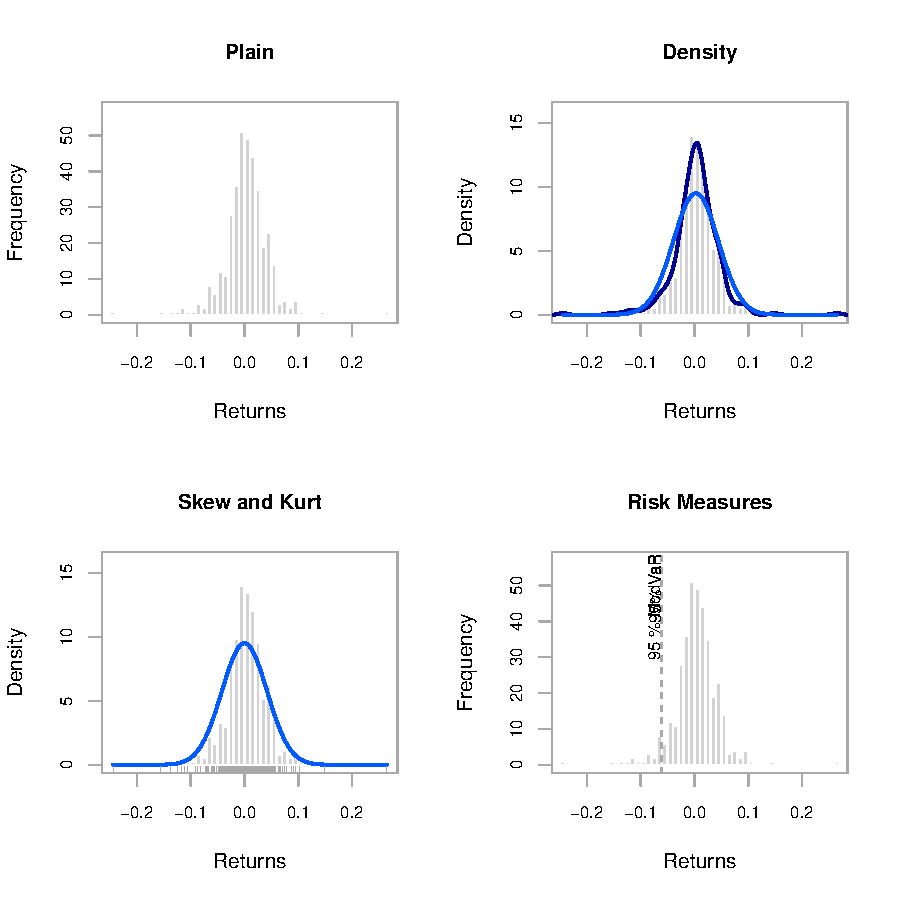
\includegraphics{graphics/plot-003}

\section{All yr Performance}
\setkeys{Gin}{width=0.5\textwidth}
%\begin{landscape}
\subsection{Returns}
\begin{tabular}{cc}
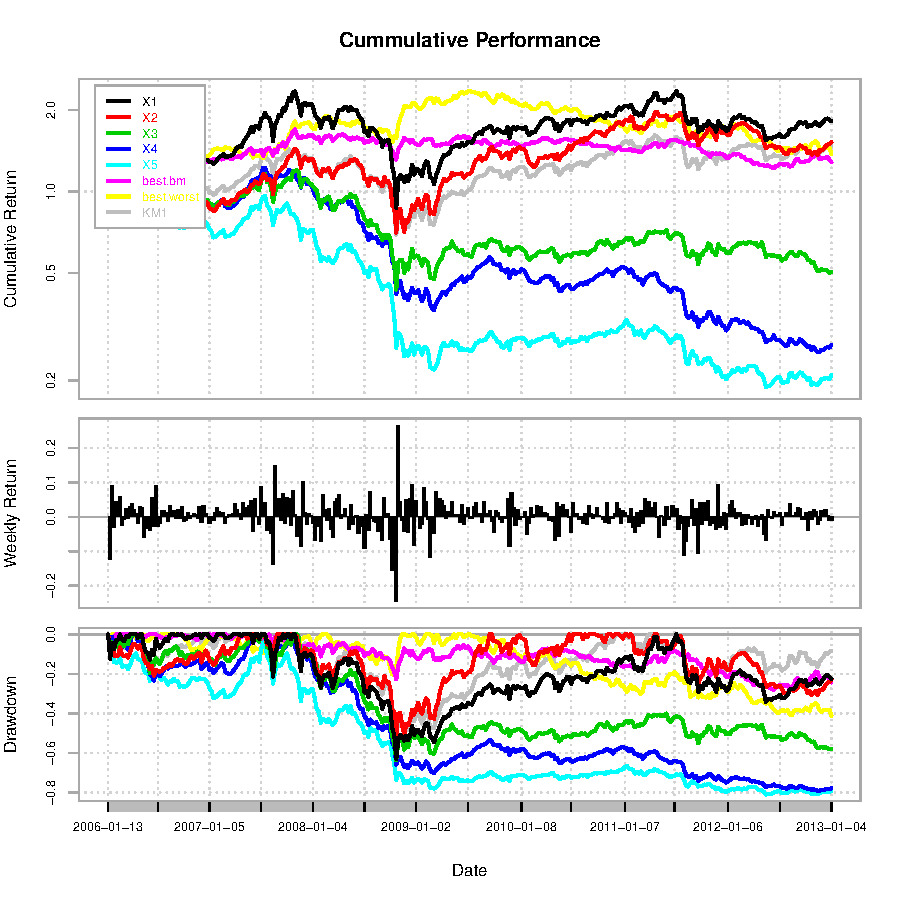
\includegraphics{graphics/plot-004}
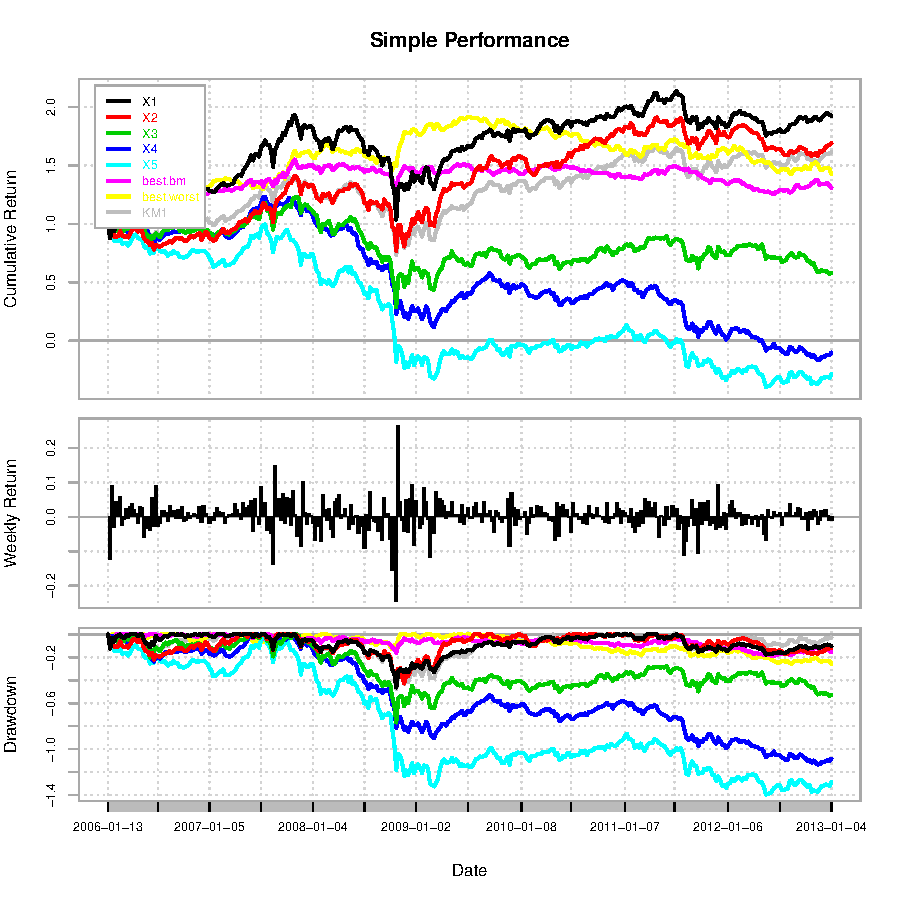
\includegraphics{graphics/plot-005}
\end{tabular}

%\end{landscape}
\subsection{Relative Returns}
\begin{tabular}{cc}
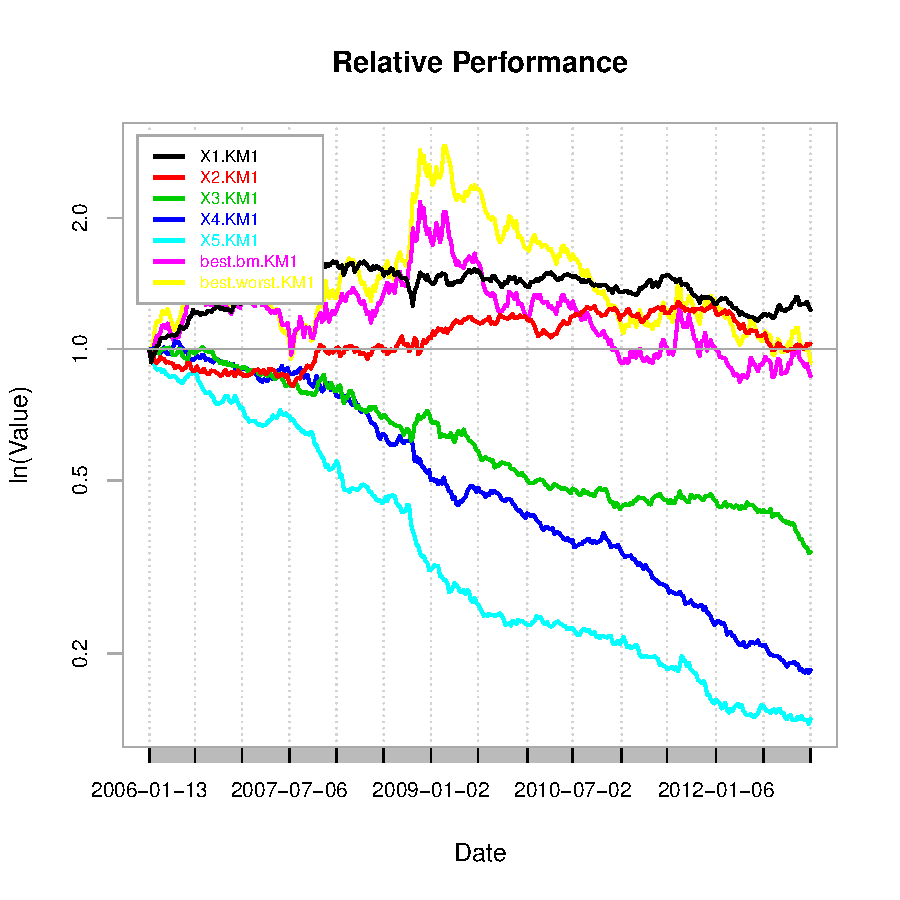
\includegraphics{graphics/plot-006}
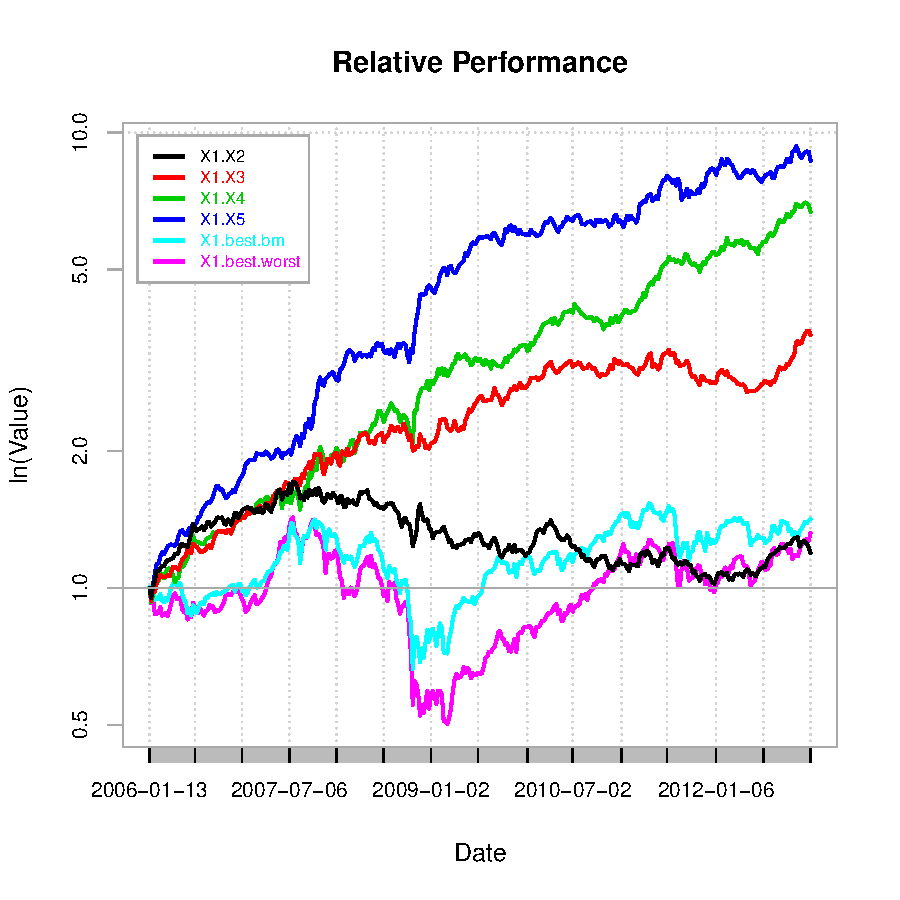
\includegraphics{graphics/plot-007}
\end{tabular}
\subsection{Other Charts}
\begin{tabular}{cc}
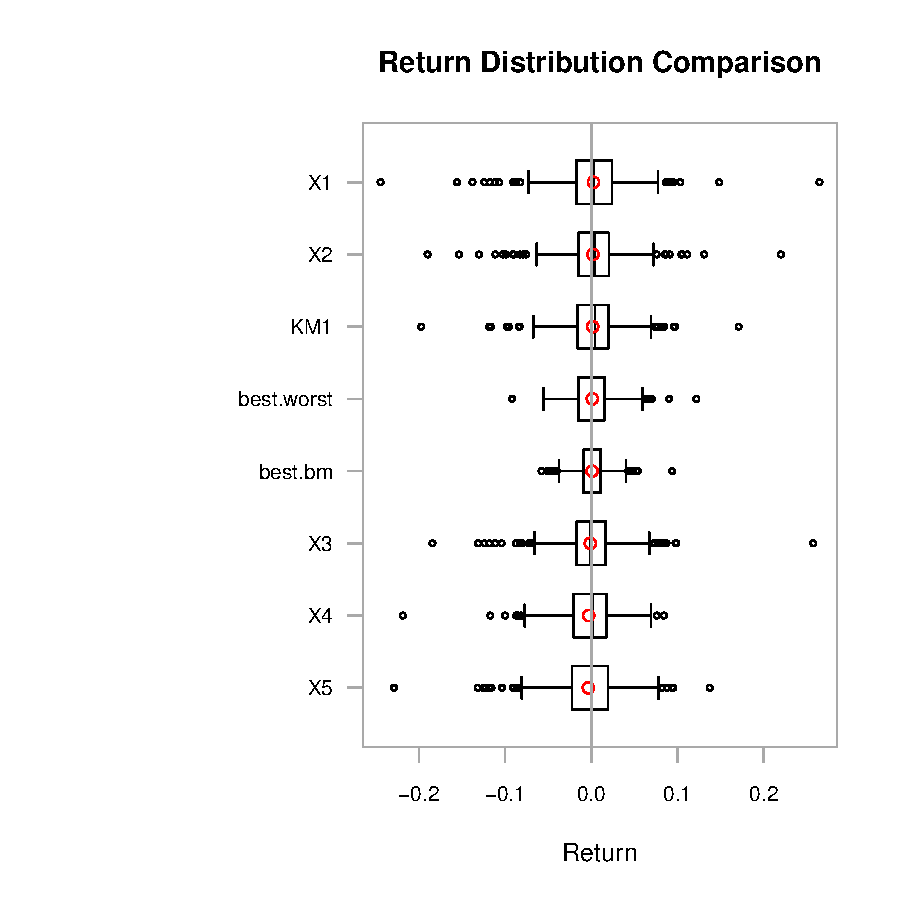
\includegraphics{graphics/plot-008}
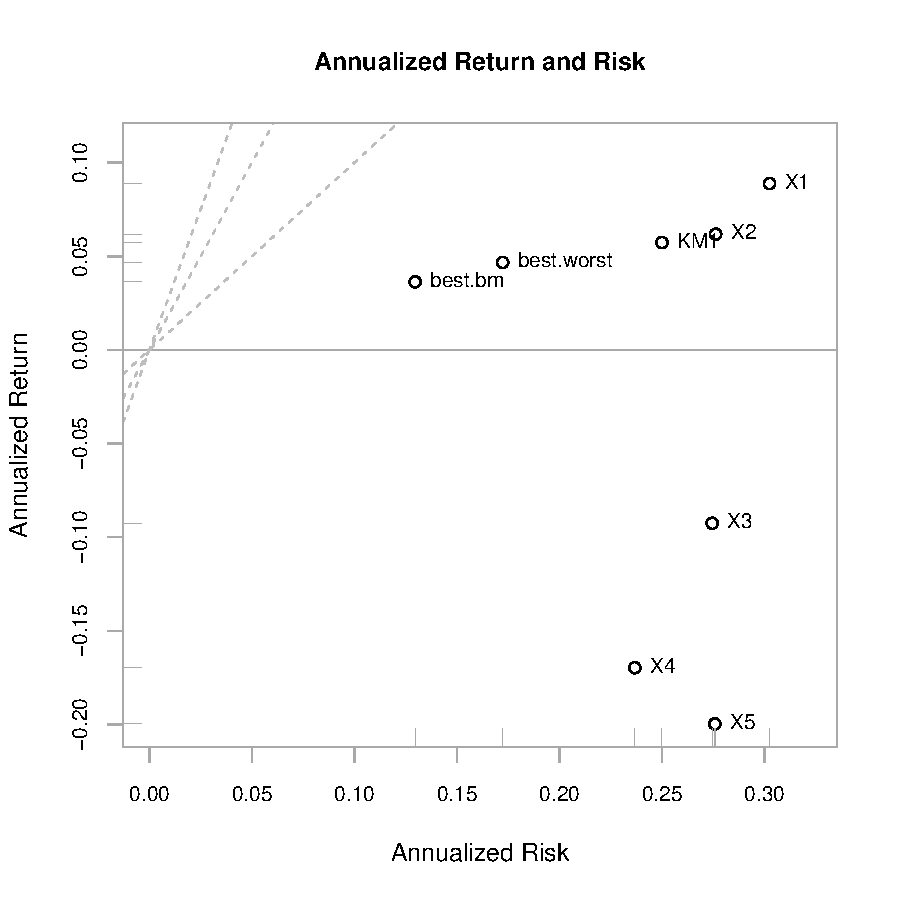
\includegraphics{graphics/plot-009}
\end{tabular}
\section{3yr Performance}
%\begin{landscape}
\subsection{Returns}
\begin{tabular}{cc}
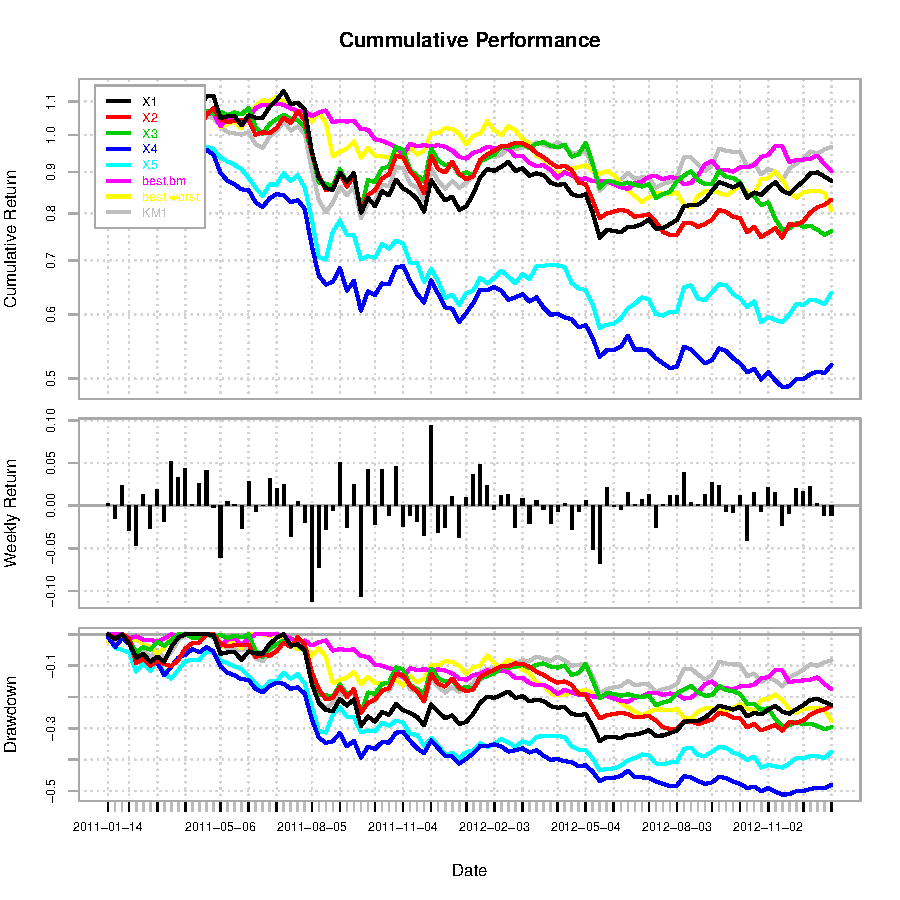
\includegraphics{graphics/plot-010}
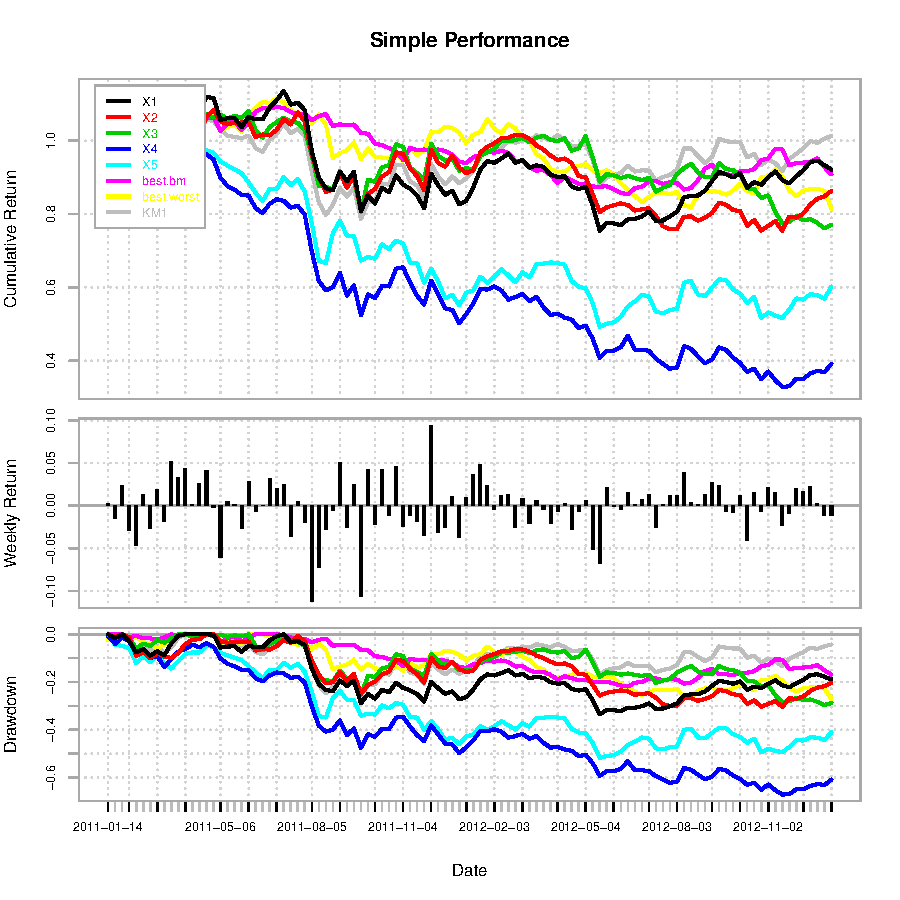
\includegraphics{graphics/plot-011}
\end{tabular}
%\end{landscape}
\subsection{Relative Returns}
\begin{tabular}{cc}
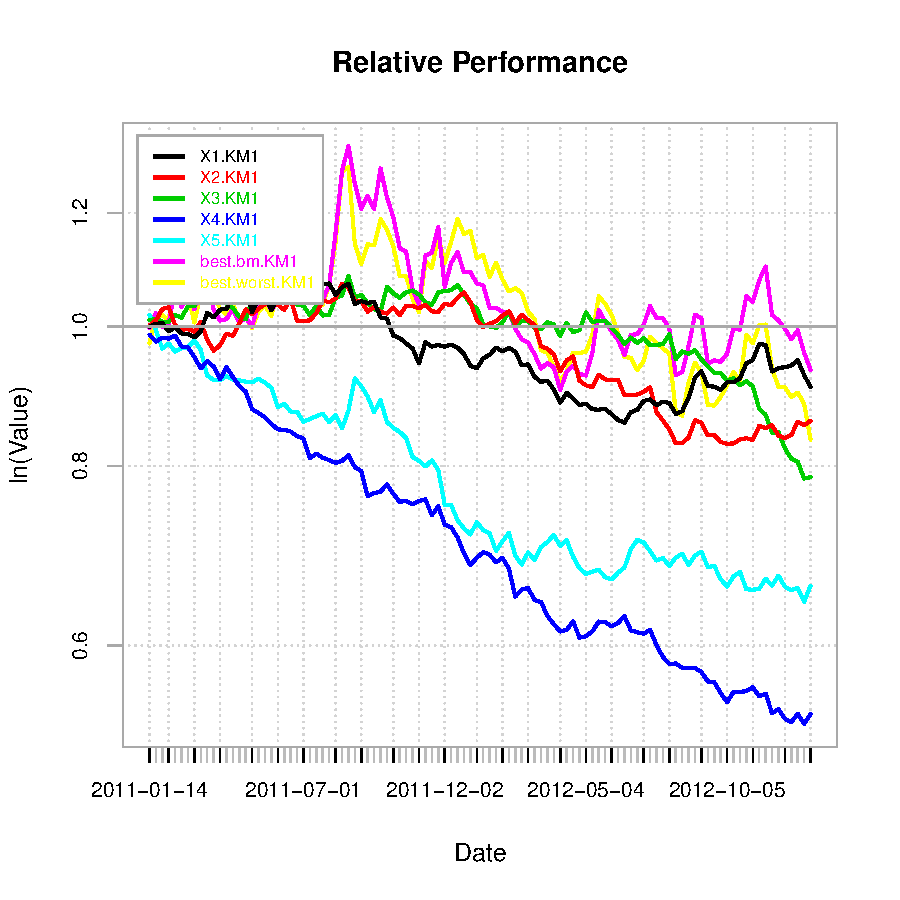
\includegraphics{graphics/plot-012}
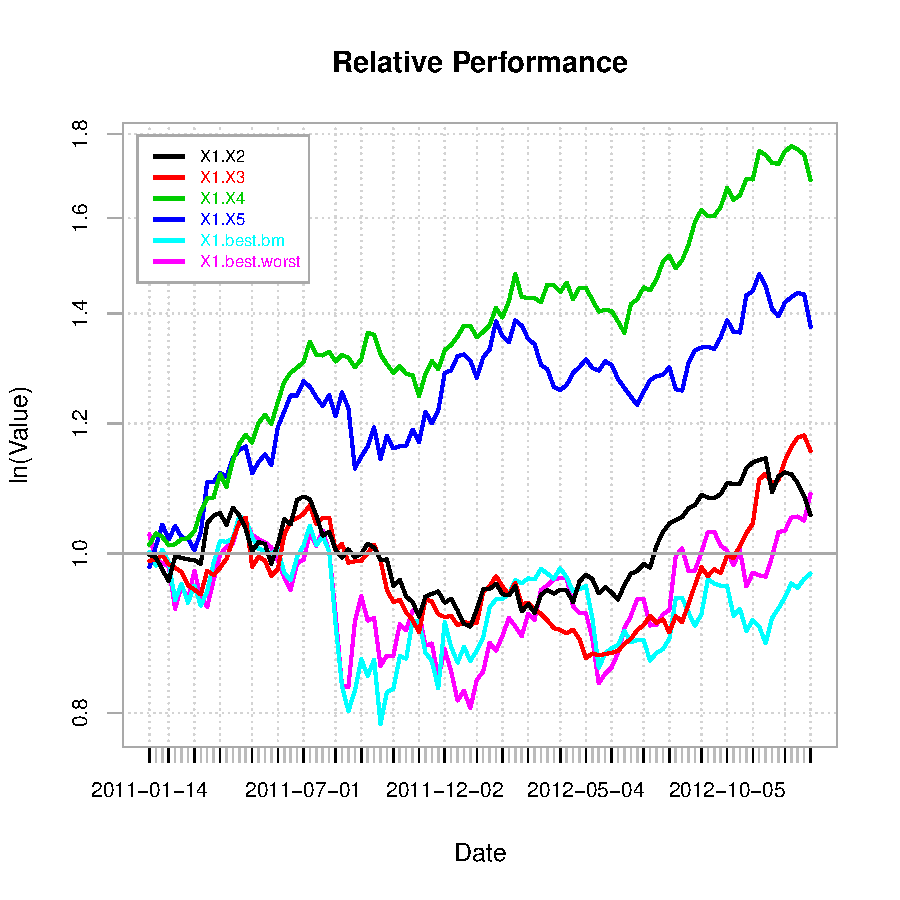
\includegraphics{graphics/plot-013}
\end{tabular}
\subsection{Other Charts}
\begin{tabular}{cc}
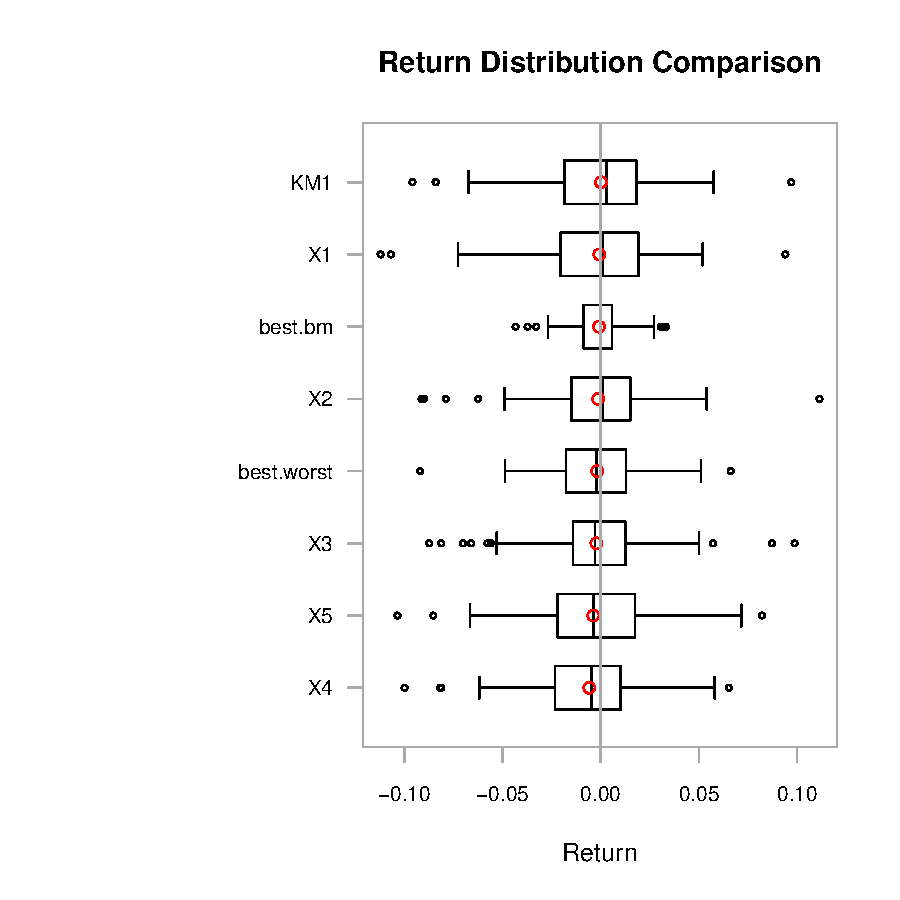
\includegraphics{graphics/plot-014}
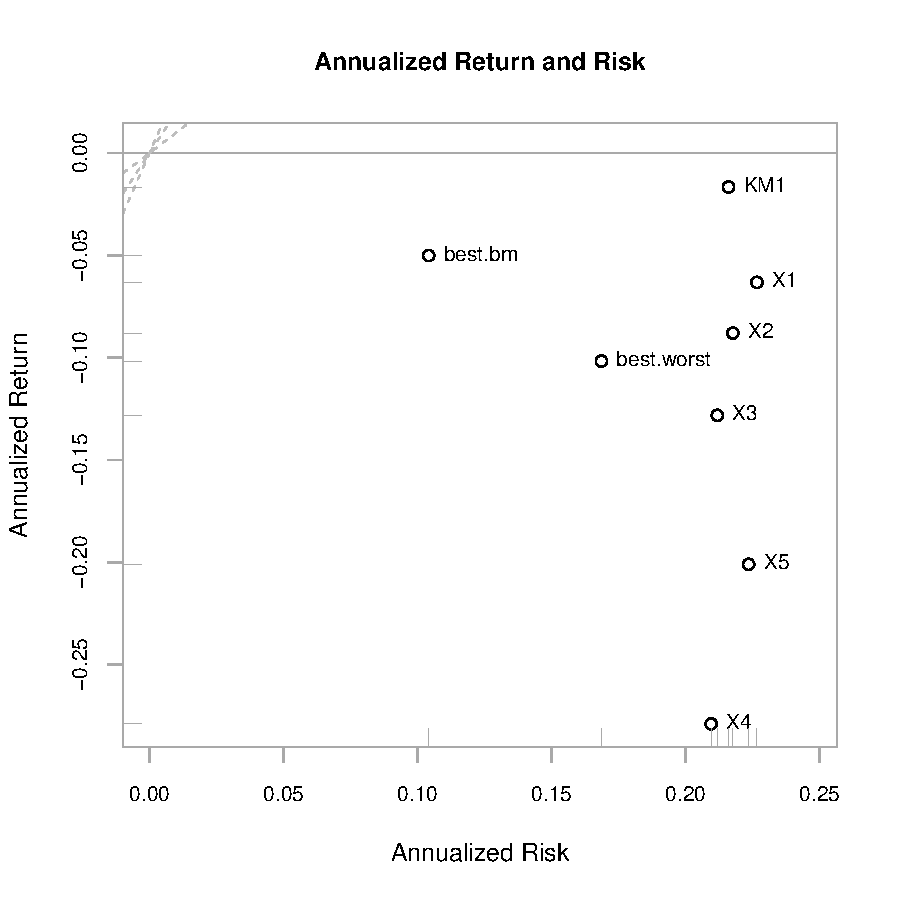
\includegraphics{graphics/plot-015}
\end{tabular}
\section{1yr Performance}
%\begin{landscape}
\subsection{Returns}
\begin{tabular}{cc}
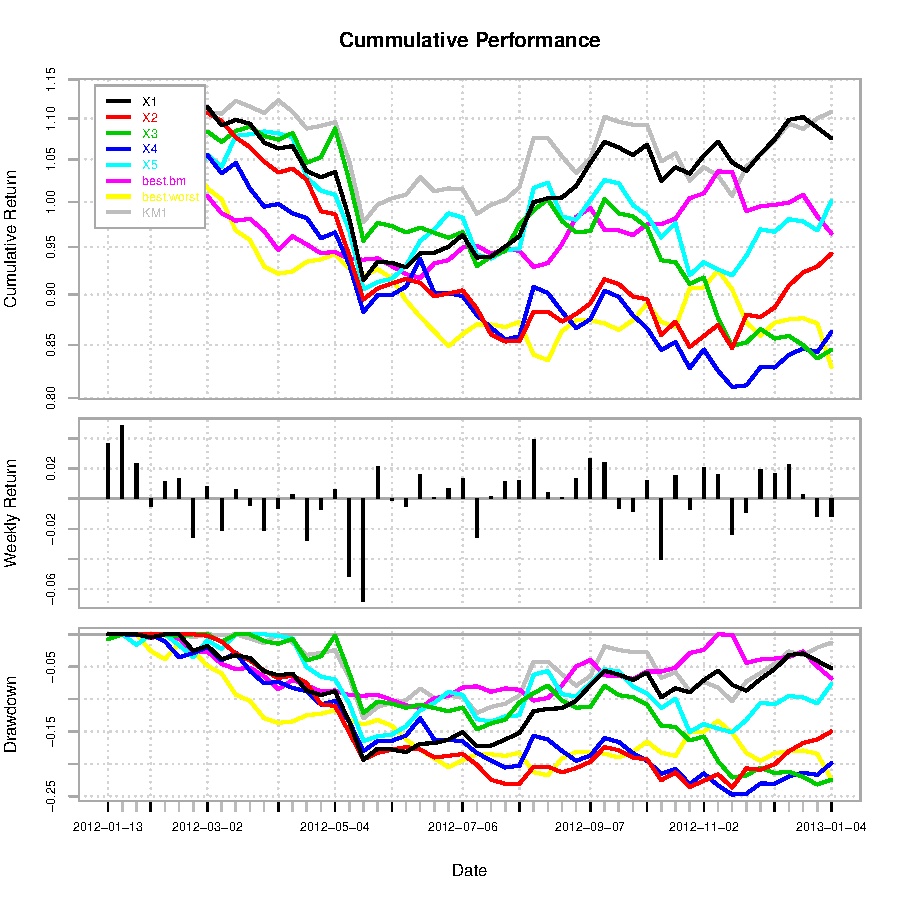
\includegraphics{graphics/plot-016}
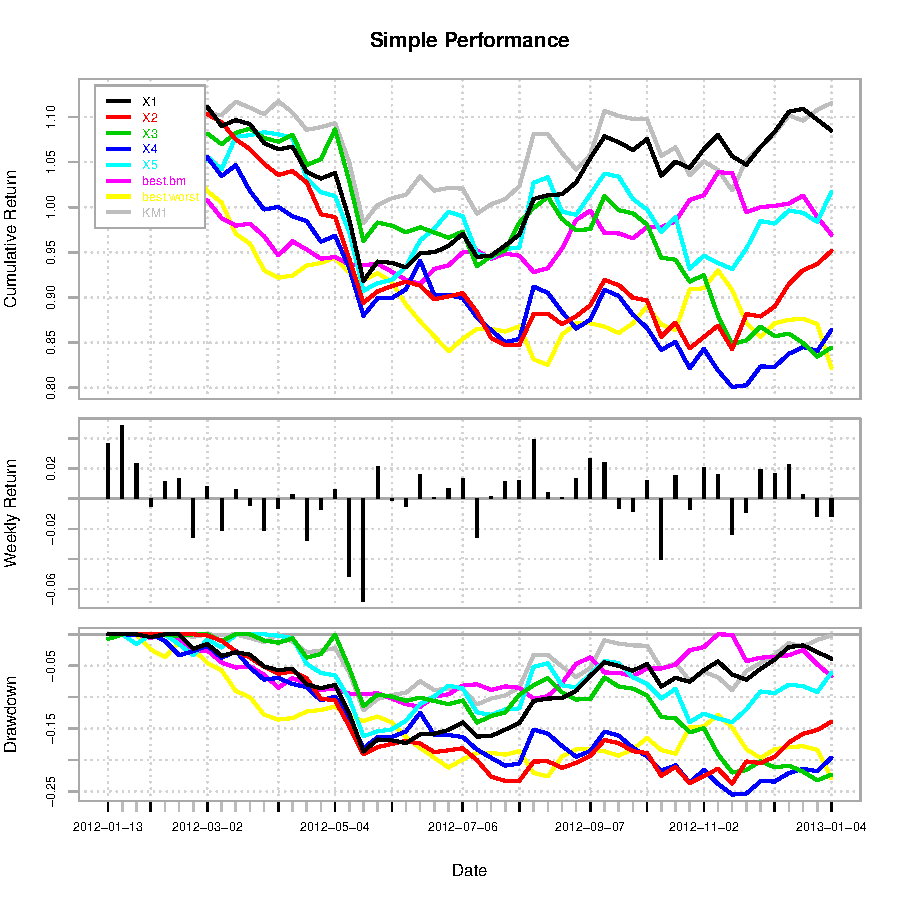
\includegraphics{graphics/plot-017}
\end{tabular}
%\end{landscape}
\subsection{Relative Returns}
\begin{tabular}{cc}
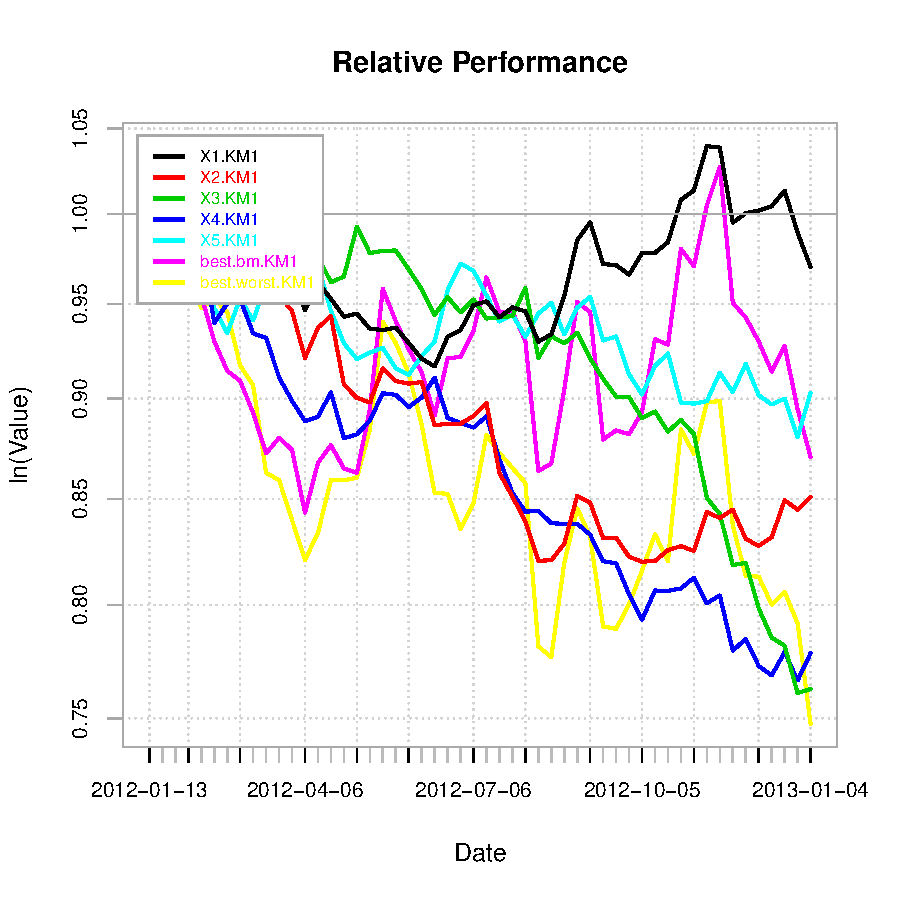
\includegraphics{graphics/plot-018}
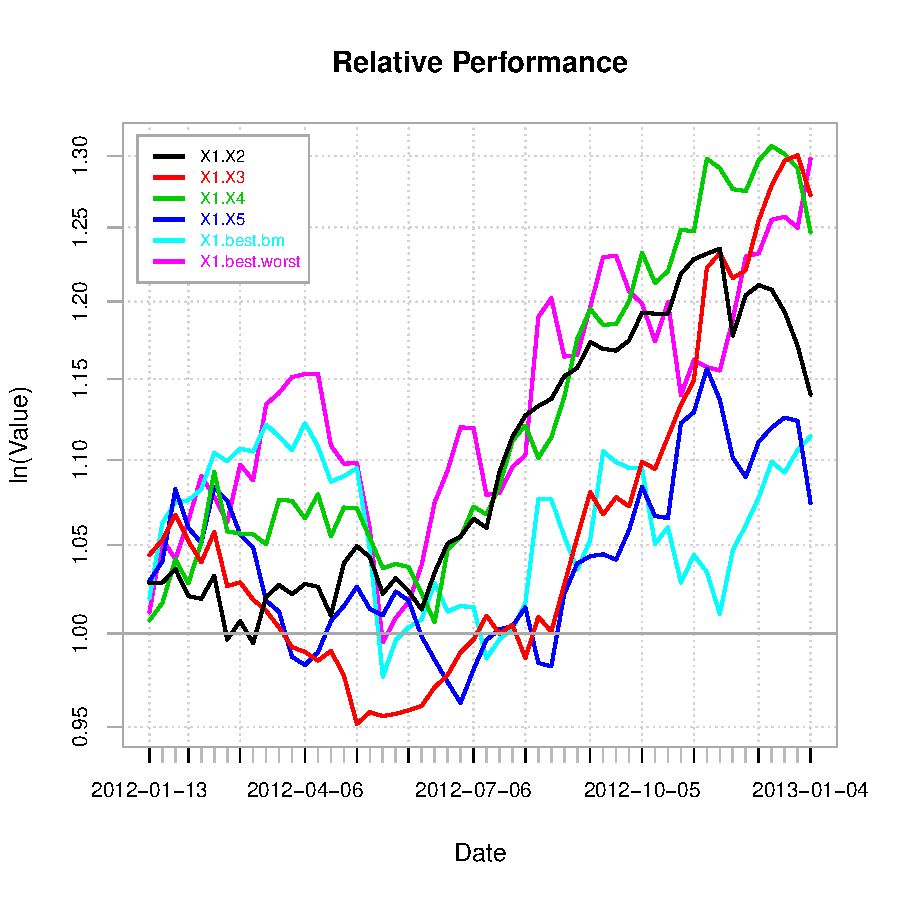
\includegraphics{graphics/plot-019}
\end{tabular}
\subsection{Other Charts}
\begin{tabular}{cc}
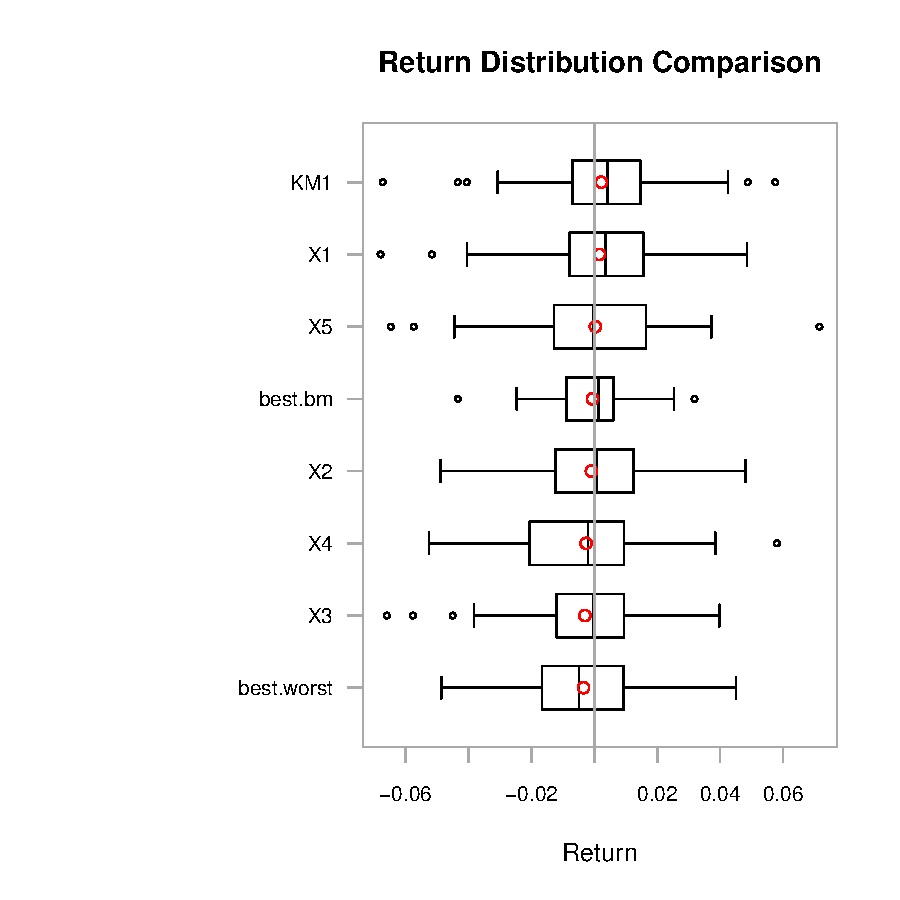
\includegraphics{graphics/plot-020}
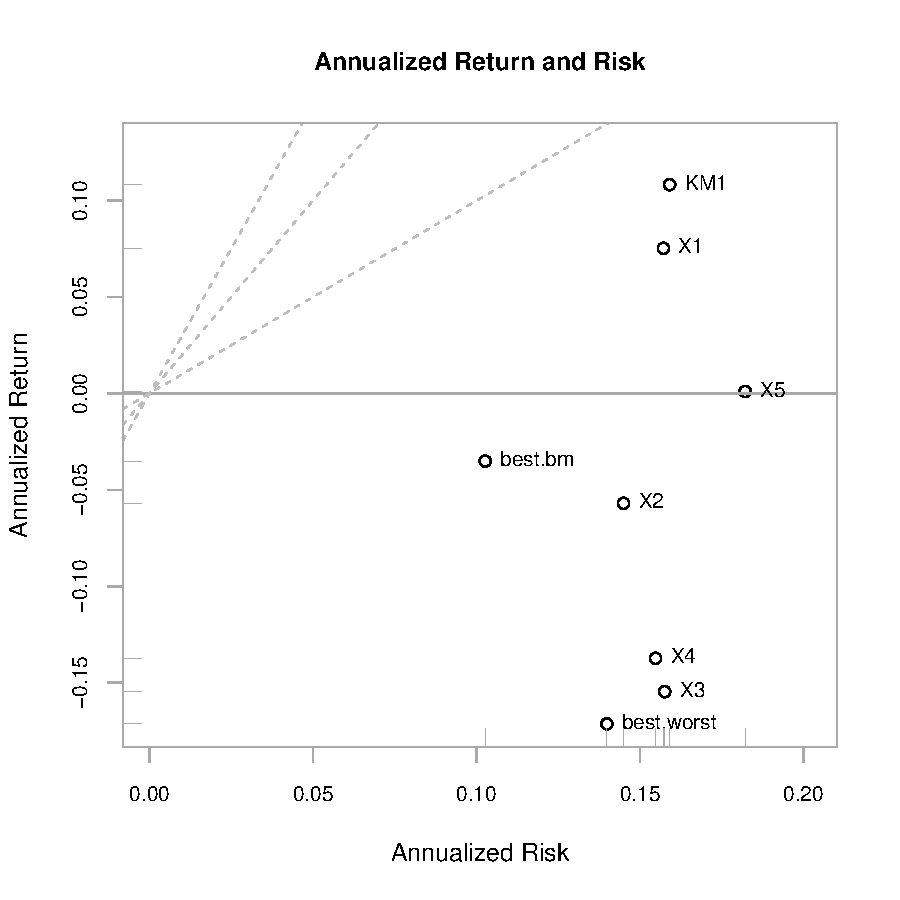
\includegraphics{graphics/plot-021}
\end{tabular}

\end{document}
